\section{Exploration and Analysis}
    \subsection{What makes a movie successful?}
        % We would like you to explore what makes a movie popular and/or successful.
        \paragraph{}
            In order to ascertain which factors are most influential in determining the
                success of a movie, it is necessary to first define what constitutes success.
            For the purpose of this analysis, success is defined as the movie's revenue.
            By examining the correlations between the movie's revenue and other factors, we
                can gain insight into which factors have the greatest impact on the success of
                a movie.
            These correlations are visualised in Figure \ref{fig-heatmap}.

            \begin{figure}[H]
                \centering
                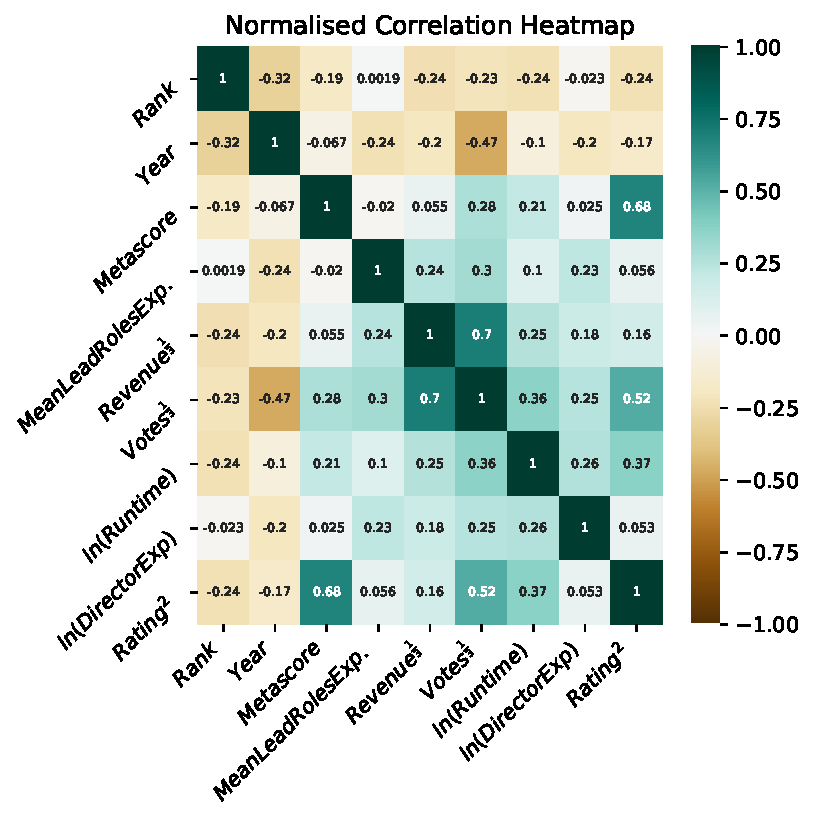
\includegraphics[width=0.8\linewidth]{Final/Normalised Correlation Heatmap.pdf}
                \caption[short]{
                    A heatmap illustrating the strength of correlations between various normalised
                    variables from the IMDb dataset \cite{data:IMDb}.
                    The Pearson's Product Moment Correlation Coefficient is used to calculate the
                        strength of the correlations.
                    These variables included Rank, Year, Metascore, Revenue, Votes, Runtime, and
                        Rating.
                    Additionally, two more variables were calculated from the TMD data
                        \cite{data:TMD}: MeanLeadRolesExperience and DirectorExperience.
                    Each correlation is represented by a value between -1 and 1, with weaker
                        correlations having values closer to 0, and negative correlations having
                        negative values and positive correlations having positive values.
                }\label{fig-heatmap}
            \end{figure}

        \paragraph{}
            Figure \ref{fig-heatmap} reveals a strong positive correlation (0.7) between a
                movie's revenue and the number of votes it receives on IMDb, suggesting that
                the more votes a movie receives, the higher its revenue is likely to be.
            Additionally, the heatmap shows moderate positive correlations between the
                movie's revenue and its runtime (0.25) and between the movie's revenue and the
                experience of the actors in lead roles (0.24), indicating that longer runtimes
                and more experienced actors may be associated with higher revenues.
            In contrast, there is a moderate negative correlation between a movie's revenue
                and its rank on IMDb (-0.24), suggesting that higher ranks on IMDb do not
                necessarily translate to higher revenues.
            These four correlations are shown in more detail in Figure
                \ref{fig-revenue-factors}.

            \begin{figure}[H]
                \centering
                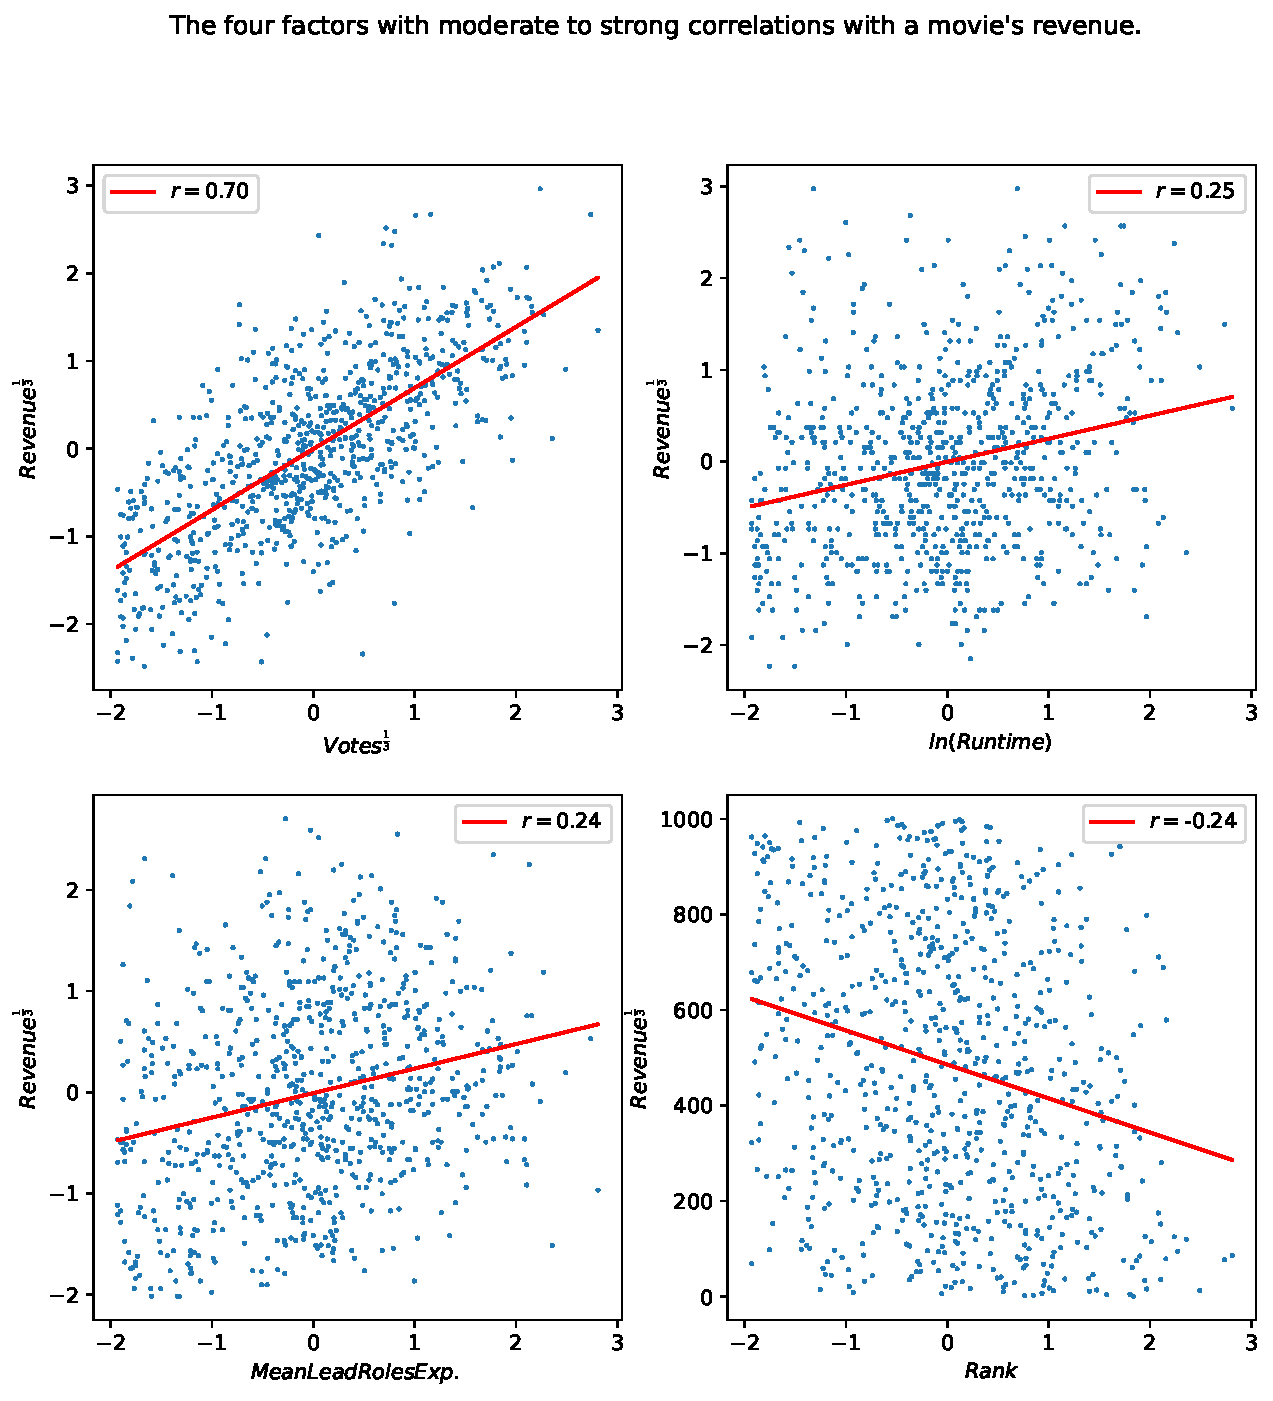
\includegraphics[width=0.8\linewidth]{Final/Revenue Factors.pdf}
                \caption[short]{
                    Scatter plots showing the relationships between a movie's revenue and the four
                    factors with moderate or strong correlations.
                }\label{fig-revenue-factors}
            \end{figure}

    \subsection{The relationship between a movie's ranked position and its number of votes}
        % We would also like you to visualise the distribution of ranked position and
        % number of votes, and comment on the relationship between them.
        \paragraph{}

    % Suggested 500 words for individual report; proportionately longer for group
    % projects).
    % Revenue Multiple Regression
    \subsection{What factors can predict box office success?}
    % We would like you to explore what makes a movie popular and/or successful.
        \paragraph{}
        In order to further analyze the correlations between the various movie details
        and the revenue they generated, we created a multiple regression model using the
        normalized data we collected. 
        The target variable was the normalised revenue, with the rest of the dataset as the 
            predictor variables, excluding Genre and Title.
        $Votes^\frac{1}{3}$ was excluded as it is causally linked to Revenue; the more votes, the more people bought movie tickets. 
        The model uses Ordinary Least Squares regression and a constant column has been added to show y-intercept.
        The summary results are provided in Table \ref{tab-revenue-ols-summary}.
        \begin{table}[H]
            \begin{center}
                \begin{tabular}{lclc}
                    \toprule
                    \textbf{Dep. Variable:}           &  $Revenue^{\frac{1}{3}}$   & \textbf{  R-squared:         } &     0.404   \\
                    \textbf{Model:}                   &       OLS        & \textbf{  Adj. R-squared:    } &     0.393   \\
                    \textbf{Method:}                  &  Least Squares   & \textbf{  F-statistic:       } &     36.60   \\
                    \textbf{No. Observations:}        &         826      & \textbf{  Prob (F-statistic):} &  1.35e-80   \\
                    \textbf{Df Residuals:}            &         810      & \textbf{Df Model:}             &       15  \\
                    \bottomrule
                \end{tabular}
                \begin{tabular}{lcccccc}
                                                    & \textbf{coef} & \textbf{std err} & \textbf{t} & \textbf{P$> |$t$|$} & \textbf{[0.025} & \textbf{0.975]}  \\
                    \midrule
                    \textbf{$const$}                &     114.0116  &       19.712     &     5.784  &         0.000        &       75.319    &      152.705     \\
                    \textbf{$Rank$}                 &      -0.0006  &        0.000     &    -5.654  &         0.000        &       -0.001    &       -0.000     \\
                    \textbf{$Year$}                 &      -0.0565  &        0.010     &    -5.770  &         0.000        &       -0.076    &       -0.037     \\
                    \textbf{$Metascore$}            &       0.0416  &        0.038     &     1.093  &         0.275        &       -0.033    &        0.116     \\
                    \textbf{$Mean Lead Roles Exp.$} &       0.1125  &        0.030     &     3.793  &         0.000        &        0.054    &        0.171     \\
                    \textbf{$ln(Runtime)$}          &       0.1705  &        0.033     &     5.203  &         0.000        &        0.106    &        0.235     \\
                    \textbf{$ln(Director Exp)$}     &       0.0507  &        0.029     &     1.756  &         0.079        &       -0.006    &        0.107     \\
                    \textbf{$Rating^2$}             &       0.0816  &        0.041     &     2.013  &         0.044        &        0.002    &        0.161     \\
                    \textbf{$Action$}               &       0.1824  &        0.070     &     2.598  &         0.010        &        0.045    &        0.320     \\
                    \textbf{$Adventure$}            &       0.4765  &        0.074     &     6.452  &         0.000        &        0.332    &        0.621     \\
                    \textbf{$Sci-Fi$}               &       0.0318  &        0.087     &     0.364  &         0.716        &       -0.140    &        0.203     \\
                    \textbf{$Thriller$}             &      -0.0395  &        0.078     &    -0.504  &         0.615        &       -0.193    &        0.114     \\
                    \textbf{$Comedy$}               &       0.1145  &        0.072     &     1.599  &         0.110        &       -0.026    &        0.255     \\
                    \textbf{$Drama$}                &      -0.5579  &        0.071     &    -7.877  &         0.000        &       -0.697    &       -0.419     \\
                    \textbf{$Romance$}              &      -0.0243  &        0.084     &    -0.288  &         0.773        &       -0.190    &        0.141     \\
                    \textbf{$Crime$}                &      -0.0545  &        0.082     &    -0.664  &         0.507        &       -0.216    &        0.107     \\
                    \bottomrule
                \end{tabular}
            \end{center}
            \caption[short]{Multiple regression results with $Revenue^{\frac{1}{3}}$ as the dependent variable
                            and the normalised data as the independent variable. The OLS approach was used to
                            find the best fit. The residuals for this model are shown in 
                            fig \ref{fig-revenue-ols-residuals}}\label{tab-revenue-ols-summary}
        \end{table}
        This model performs respectably, explaining about  40\% of the variance in box office success.
        It is also statistically significant ($R^2=0.404, F(15,810)=36.6, p<0.05$).
        The results indicate a well performing model, and as such we can postulate 
            that at least some of these factors are impactful on the box office success a movie has.

        % Director vs Actor for selling tickets
        The results suggest that box office sales can be predicted by lead actor experience ($\beta=0.113, \sigma=0.030, p<0.05$),
            but cannot be predicted by director experience ($\beta=0.051, \sigma=0.030, p>0.05$).
        Previous research has shown that movie advertising tends to be focussed around the actors 
            present more than the director of the movie\cite{elberse2007power}.
        Examples of this are present in adverts like movie posters - actor faces feature front and 
            center while directors are listed in name only.
        Actors who have been in many movies are more recognisable, meaning potential consumers
            will be more likely to invest money in seeing a movie they are part of.

        % Meta score vs Rating
        The results also suggest that box office sales can't be predicted by critics (Metascore) 
            ($\beta=0.042, \sigma=0.038, p>0.05$), but can be predicted by user rating.
            ($\beta=0.082, \sigma=0.041, p<0.05$).
        It is reasonable to assume both would have similar quality as predictor variables - they 
            correlate strongly (see fig \ref{fig-heatmap}).
        As such, the difference in quality is surprising.
        This difference could be due to movies appearing in the box office for only a short period.
        Revenue is only calculated during this period, a period of time where consumers may 
            rely on friends rather than a critics review, as those often come out later.
        With this in mind, it is reasonable to say that critics do not appear to be able to predict the likelihood
            of a movie becoming a blockbuster.
        
        % Genre notes
        Finally, there are some interesting notes about the impact of genre has on the box office success of a movie.
        Adventure seems to have the biggest positive impact on box office success ($\beta=0.477,\sigma=0.074,p<0.05$).
        Dramas appear to have the largest negative impact on box office success ($\beta=-0.558,\sigma=0.071,p<0.05$).
    \subsection{Can critics truly predict movie success?}
        % We would like you to explore what makes a movie popular and/or successful.
        \paragraph{}
        % Success metric definition
        To analyze the effect critics had on predicting general success of a movie, we define
            a metric of success, $Success = \frac{Revenue^\frac{1}{3} + Rating^2}{2}$.
        We chose this metric as Revenue and Rating are both measures of movie success,
            and Figure \ref{fig-heatmap} shows that they are not strongly correlated.
        This means they describe independent aspects of success, and therefore the mean of both
            will better encapsulate the true success of a movie.
        We refer to this metric as success from now on.
        
        To investigate the ability for critics to predict movie success, we present a multiple regression model,
            with the target variable being the success metric. 
        We used the rest of the normalised dataset for predictor variables, excluding the $Revenue^\frac{1}{3}$, $Rating^2$,
            Genre and Title columns.
        Genre and Title were excluded as they are not quantative data and $Revenue^\frac{1}{3}$ and $Rating^2$ were excluded
            as they are causally  linked to the success metric.
        We use the same approach as in Table \ref{tab-revenue-ols-summary}, with a constant column and using OLS.
        The summary results are provided in Table \ref{tab-success-ols-summary}.
        \begin{table}[H]
            \begin{center}
                \begin{tabular}{lclc}
                    \toprule
                    \textbf{Dep. Variable:}           &     Success      & \textbf{  R-squared:         } &     0.758   \\
                    \textbf{Model:}                   &       OLS        & \textbf{  Adj. R-squared:    } &     0.753   \\
                    \textbf{Method:}                  &  Least Squares   & \textbf{  F-statistic:       } &     169.1   \\
                    \textbf{No. Observations:}        &         826      & \textbf{  Prob (F-statistic):} & 2.67e-237   \\
                    \textbf{Df Residuals:}            &         810      & \textbf{Df Model:}             &       14     \\
                    \bottomrule
                \end{tabular}
                \begin{tabular}{lcccccc}
                                                    & \textbf{coef} & \textbf{std err} & \textbf{t} & \textbf{P$> |$t$|$} & \textbf{[0.025} & \textbf{0.975]}  \\
                    \midrule
                    \textbf{$const$}                &     -49.4262  &       10.871     &    -4.547  &         0.000        &      -70.765    &      -28.087     \\
                    \textbf{$Rank$}                 &      -0.0001  &     5.42e-05     &    -2.173  &         0.030        &       -0.000    &    -1.14e-05     \\
                    \textbf{$Year$}                 &       0.0246  &        0.005     &     4.560  &         0.000        &        0.014    &        0.035     \\
                    \textbf{$Metascore$}            &       0.1858  &        0.015     &    12.006  &         0.000        &        0.155    &        0.216     \\
                    \textbf{$Mean Lead Roles Exp.$} &      -0.0003  &        0.015     &    -0.022  &         0.983        &       -0.029    &        0.028     \\
                    \textbf{$Votes^{\frac{1}{3}}$}  &       0.5669  &        0.020     &    28.674  &         0.000        &        0.528    &        0.606     \\
                    \textbf{$ln(Runtime)$}          &       0.0820  &        0.016     &     5.185  &         0.000        &        0.051    &        0.113     \\
                    \textbf{$ln(Director Exp)$}     &      -0.0318  &        0.014     &    -2.286  &         0.023        &       -0.059    &       -0.004     \\
                    \textbf{$Action$}               &      -0.0532  &        0.034     &    -1.561  &         0.119        &       -0.120    &        0.014     \\
                    \textbf{$Adventure$}            &       0.1279  &        0.036     &     3.554  &         0.000        &        0.057    &        0.199     \\
                    \textbf{$Sci-Fi$}               &      -0.2271  &        0.043     &    -5.300  &         0.000        &       -0.311    &       -0.143     \\
                    \textbf{$Thriller$}             &      -0.0610  &        0.038     &    -1.610  &         0.108        &       -0.135    &        0.013     \\
                    \textbf{$Comedy$}               &       0.0376  &        0.035     &     1.087  &         0.277        &       -0.030    &        0.106     \\
                    \textbf{$Drama$}                &      -0.0391  &        0.035     &    -1.133  &         0.258        &       -0.107    &        0.029     \\
                    \textbf{$Romance$}              &      -0.0858  &        0.041     &    -2.103  &         0.036        &       -0.166    &       -0.006     \\
                    \textbf{$Crime$}                &      -0.0795  &        0.040     &    -2.003  &         0.046        &       -0.157    &       -0.002     \\
                    \bottomrule
                \end{tabular}
            \end{center}
        \caption[short]{Multiple regression results with $Revenue^{\frac{1}{3}}$ as the dependent variable
                        and the normalised data as the independent variable. The OLS approach was used to
                        find the best fit. The residuals for this model are shown in 
                        fig \ref{fig-success-ols-residuals}}\label{tab-success-ols-summary}
        \end{table}
    This model performs very well, explaining about 75\% of the variance in user ratings.
        It is also statistically significant ($R^2=0.758, F(14,810)=169, p<0.05$).
    The results indicates a well performing model, and as such we can postulate 
        that at least some of these factors are impactful on the success a movie has.

    % Metascore analysis
    The results show that movie success can be well predicted by Metascore ($\beta=0.186, \sigma=0.015, p<0.05$).
    This compares to how it is not a good predictor of Revenue (see Table \ref{tab-revenue-ols-summary}).
    This difference shows that while critics can't predict the box office success, they can predict the 
        overall success of the movie.
    Metascore is one of the key predictors in this model - with the third largest absolute coefficient - 
        demonstrating that critics are important when it comes to predicting the success of a movie.
    This idea is supported by the PPMCC that Metascore has with the Success metric ($R^2=0.48$).
    This is a relatively strong correlation, suggesting that critics can discern potentially successful movies.
    
    % Constant
    Another observation is the constants coefficient is negative ($\beta=-49.4,\sigma=10.9,p<0.05$).
    This means that the average movie tends to not be very successful, which is inline with research that
        most movies do not succeed, with only a few actually garnering actual success \cite{walls2005modelling}.

    % Genre notes
    Finally, there are some interesting notes about the impact of genre has on the box office success of a movie.
    Adventure seems to have the biggest positive impact on success ($\beta=0.128,\sigma=0.036,p<0.05$).
    Sci-Fi appears to have the largest negative impact on success ($\beta=-0.223,\sigma=0.043,p<0.05$).

\begin{figure}[H]
    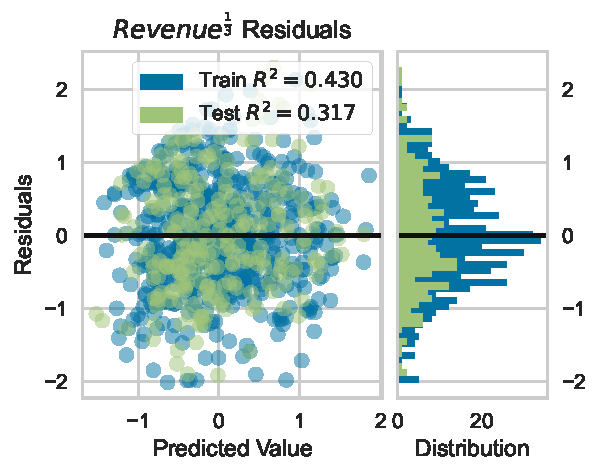
\includegraphics[width=\linewidth]{/Final/Revenue OLS Residuals.pdf}
    \caption[short]{title}\label{fig-revenue-ols-residuals}
\end{figure}

\begin{figure}[H]
    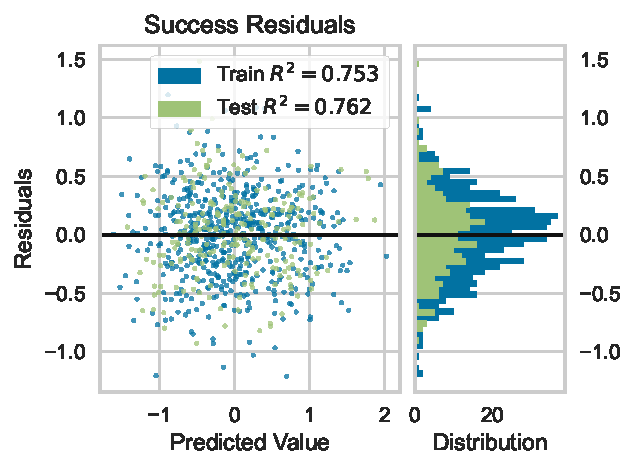
\includegraphics[width=\linewidth]{/Final/Success OLS Residuals.pdf}
    \caption[short]{title}\label{fig-success-ols-residuals}
\end{figure}
